\documentclass[../main.tex]{subfiles}

\begin{document}

    \chapter{Introduction}

    \section{Error detection and correction}
    When data is stored or transmitted, we cannot ignore encoding. The field of mathematics that deals with sending data, a digital bit stream, over a noisy channel is called coding theory. The Oxford English Dictionary says the following about code:

    \begin{quote}
        Any system of symbols and rules for expressing information or instructions in a form usable by a computer or other machine for processing or transmitting information.
    \end{quote}

    \paragraph{}
    During World War II, and even before, as far back as classic times, messages had to be send to allies but it was crucial they were unintelligible to the enemy. This field of cryptology was born out of necessity, a sense of survival. After the war, before governments could render the research obsolete, the people behind cryptology research showed that cryptology and eventually the theory of error detecting and correcting could be put into practical use. We can see that the field of cryptology is adjacent to and often-times overlapping with the field of coding theory (Trappe \& Washington 2006).

    \paragraph{}
    This thesis will briefly look at some pioneers and their achievements, then goes through the basics of coding theory and addresses the mathematics behind coding in chapter 2. While chapter 3 goes into the theory of linear block codes, it will be the visualisation in chapter 4 that explains how burst errors can be detected and corrected, on e.g. a Compact Disc. Physical damage like dust or scratches or material impurities can cause erasures or burst errors in the data stream. With forward error correction techniques like Reed-Solomon codes these interrupts in the data stream can be detected and corrected.


    \section{History of Error Control Coding}
    Pioneers of coding theory are Shannon, Hamming who were colleagues at Bell Labs. Hocquenghem in 1959 and independently Bose and Ray-Chaudhuri in 1960 were responsible for a class of codes known an BCH codes. Reed and Solomon followed with a set of cyclic codes, which are BCH codes, but are well suited for detecting and correcting burst errors and erasures. It wasn't until almost a decade later when Berlekamp invented a decoding algorithm which was simplified by Massey in 1969. In 1982 the Compact Disc (CD) was the first mass-produced device that used these error correcting codes.


    \subsection{Shannon}
    Claude Shannon (1916–2001) was an electronic engineer and mathematician and during the Second World War he joined Bell Labs to work on cryptography. His work was closely related to coding theory and eventually led to publication of the article named A Mathematical Theory of Communication in 1948, which is now regarded as one of the founding works of communication theory. Presently, not only do many regard him as the father of information theory, but he is also credited with establishing digital computer and digital circuit design theory while he was a master's student at MIT (Bose 2008).


    \subsection{Hamming}
    Richard Hamming (1915–1998) was a contemporary and colleague of Shannon at Bell Labs. While doing research on cryptology, Hamming became interested in the idea of error correcting codes while working on a relay computer out of normal office hours. Unfortunately there were no computer operators available to react to an alarm in case an error was detected. Hamming had to devise a code that would not only detect an error, but would also be able to correct it automatically, instead of just ringing the alarm. These codes are used to add redundancy to data which aid the detection and correction of errors. Chapter 3 explains the Hamming code, which was a first in the the field we now know as coding theory.

    \paragraph{}
    Although the Hamming code was referred to by Shannon in 1948, patent considerations prevented its independent publication until 1950.


    \subsection{Hocquenghem, Bose and Ray-Chaudhuri}
    Alexis Hocquenghem (1908?–1990) was a French mathematician, whose article “Codes correcteurs d'erreurs” from 1959 mentioned codes that he described as a “generalization of Hamming's work” (Hocquenghem 1959).

    \paragraph{}
    Independently from Hocquenghem, Ph.D. adviser Raj Bose (1901–1987) and his student Dwijendra Ray-Chaudhuri (1933– ) published “On a class of error correcting binary group codes” in 1960. This class of linear block codes is named after Bose, Ray-Chaudhuri and Hocquenghem and became known as BCH codes (Wicker \& Bhargava 1999).


    \subsection{Reed and Solomon}
    Irving Reed (1923– ) is an American mathematician and engineer who is best known for co-inventing a class of algebraic codes known as Reed-Solomon (RS) codes in collaboration with Gustave Solomon (1930–1996). RS codes are seen as a special case of the larger class of BCH codes but it wasn't until almost a decade later, by regarding them as cyclic BCH codes, that an efficient decoding algorithm gave them the potential to their widespread application.


    \subsection{Berlekamp and Massey}
    Elwyn Berlekamp (1940– ) is a professor emeritus of mathematics, electrical engineering and computer science at the University of California, Berkely. While he was studying electrical engineering at MIT one of his Ph.D. advisers was Claude Shannon. Berlekamp invented an algorithm for decoding BCH codes in 1968, but it was James Massey (1934– ), an information theorist and cryptographer, who simplified this algorithm in 1968 which we know as the Berlekamp-Massey algorithm (Massey 1969).

    \paragraph{}
    This algorythm made it possible to develop a fast and efficient decoder with a linear feedback shift register (LSFR), but it was not until 1982 with the advent of the mass production of the Compact Disc that the digital information age as we know it was started. Today RS codes are widely in use in many applications that involve data transmission, like computer networks: TCP/IP; telephony: GSM, GPRS, UMTS; digital video broadcasting: DVB, and data storage, like Hard-drives in computers; memory cards in cameras and telephones and optical storage like Compact Discs (CD), Digital Versitile Discs (DVD) and Blu-ray Discs (BD).


    \section{Basics of Data Communication}
    A sender transmits a message through a channel to a receiver. The channel in these cases could be air when usin a wireless network or an ethernet cable. Noise may appear on these channels, so in order to receive the message with as few errors as possible, idealy the sender should use high power signal amplification and the channel should be as short as possible. However, in normal situations however these are not viable solutions. GSM telephones have in fact very small batteries and are rather energy efficient and the ethernet cable in a building can be up to 100 meters before an active repeater or switch has to amplify the signal. In order to use as little energy as possible and transmit over a long distance, codewords have to be encoded, as shown in Illustration 1.1. It is then transmitted over a channel where errors may be introduced. The received codeword needs to be decoded into the received message.

    \begin{figure}
        \begin{center}
            \maxwidth{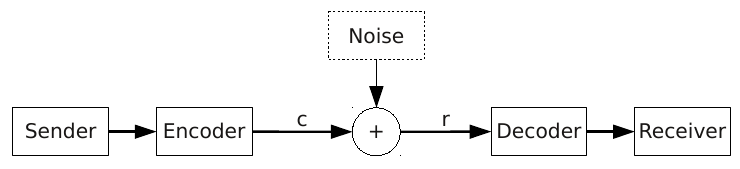
\includegraphics{digital_transmission_system}}
        \end{center}
        \caption{Digital transmission system}
    \end{figure}

    \paragraph{}
    The probability that codeword r is received if codeword c is transmitted can be expressed as P(r$|$c) . In Illustration 1.2, a model of a binary symmetric channel (BSC) shows the event that a 1 is transmitted. There is a probability that 0 is received. The transmission is unaltered with a probability of 1-p (Bossert 1999).

    \begin{figure}
        \begin{center}
            \maxwidth{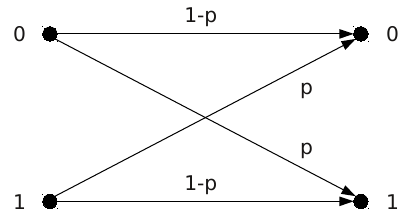
\includegraphics{binary_symmetric_channel}}
        \end{center}
        \caption{Model of the binary symmetric channel (BSC)}
    \end{figure}



\end{document}
